%%
% Copyright (c) 2017 - 2024, Pascal Wagler;
% Copyright (c) 2014 - 2024, John MacFarlane
%
% All rights reserved.
%
% Redistribution and use in source and binary forms, with or without
% modification, are permitted provided that the following conditions
% are met:
%
% - Redistributions of source code must retain the above copyright
% notice, this list of conditions and the following disclaimer.
%
% - Redistributions in binary form must reproduce the above copyright
% notice, this list of conditions and the following disclaimer in the
% documentation and/or other materials provided with the distribution.
%
% - Neither the name of John MacFarlane nor the names of other
% contributors may be used to endorse or promote products derived
% from this software without specific prior written permission.
%
% THIS SOFTWARE IS PROVIDED BY THE COPYRIGHT HOLDERS AND CONTRIBUTORS
% "AS IS" AND ANY EXPRESS OR IMPLIED WARRANTIES, INCLUDING, BUT NOT
% LIMITED TO, THE IMPLIED WARRANTIES OF MERCHANTABILITY AND FITNESS
% FOR A PARTICULAR PURPOSE ARE DISCLAIMED. IN NO EVENT SHALL THE
% COPYRIGHT OWNER OR CONTRIBUTORS BE LIABLE FOR ANY DIRECT, INDIRECT,
% INCIDENTAL, SPECIAL, EXEMPLARY, OR CONSEQUENTIAL DAMAGES (INCLUDING,
% BUT NOT LIMITED TO, PROCUREMENT OF SUBSTITUTE GOODS OR SERVICES;
% LOSS OF USE, DATA, OR PROFITS; OR BUSINESS INTERRUPTION) HOWEVER
% CAUSED AND ON ANY THEORY OF LIABILITY, WHETHER IN CONTRACT, STRICT
% LIABILITY, OR TORT (INCLUDING NEGLIGENCE OR OTHERWISE) ARISING IN
% ANY WAY OUT OF THE USE OF THIS SOFTWARE, EVEN IF ADVISED OF THE
% POSSIBILITY OF SUCH DAMAGE.
%%

%%
% This is the Eisvogel pandoc LaTeX template.
%
% For usage information and examples visit the official GitHub page:
% https://github.com/Wandmalfarbe/pandoc-latex-template
%%

% Options for packages loaded elsewhere
\PassOptionsToPackage{unicode}{hyperref}
\PassOptionsToPackage{hyphens}{url}
\PassOptionsToPackage{dvipsnames,svgnames,x11names,table}{xcolor}
%
\documentclass[
  paper=a4,
  oneside  ,captions=tableheading
]{scrartcl}
\usepackage{amsmath,amssymb}
% Use setspace anyway because we change the default line spacing.
% The spacing is changed early to affect the titlepage and the TOC.
\usepackage{setspace}
\setstretch{1.2}
\usepackage{iftex}
\ifPDFTeX
  \usepackage[T1]{fontenc}
  \usepackage[utf8]{inputenc}
  \usepackage{textcomp} % provide euro and other symbols
\else % if luatex or xetex
  \usepackage{unicode-math} % this also loads fontspec
  \defaultfontfeatures{Scale=MatchLowercase}
  \defaultfontfeatures[\rmfamily]{Ligatures=TeX,Scale=1}
\fi
\usepackage{lmodern}
\ifPDFTeX\else
  % xetex/luatex font selection
    \setmainfont[]{Inter}
    \setmonofont[]{FiraCode}
\fi
% Use upquote if available, for straight quotes in verbatim environments
\IfFileExists{upquote.sty}{\usepackage{upquote}}{}
\IfFileExists{microtype.sty}{% use microtype if available
  \usepackage[]{microtype}
  \UseMicrotypeSet[protrusion]{basicmath} % disable protrusion for tt fonts
}{}
\makeatletter
\@ifundefined{KOMAClassName}{% if non-KOMA class
  \IfFileExists{parskip.sty}{%
    \usepackage{parskip}
  }{% else
    \setlength{\parindent}{0pt}
    \setlength{\parskip}{6pt plus 2pt minus 1pt}}
}{% if KOMA class
  \KOMAoptions{parskip=half}}
\makeatother
\usepackage{xcolor}
\definecolor{default-linkcolor}{HTML}{A50000}
\definecolor{default-filecolor}{HTML}{A50000}
\definecolor{default-citecolor}{HTML}{4077C0}
\definecolor{default-urlcolor}{HTML}{4077C0}
\usepackage[margin=2.5cm,includehead=true,includefoot=true,centering,]{geometry}
\usepackage{color}
\usepackage{fancyvrb}
\newcommand{\VerbBar}{|}
\newcommand{\VERB}{\Verb[commandchars=\\\{\}]}
\DefineVerbatimEnvironment{Highlighting}{Verbatim}{commandchars=\\\{\}}
% Add ',fontsize=\small' for more characters per line
\usepackage{framed}
\definecolor{shadecolor}{RGB}{241,243,245}
\newenvironment{Shaded}{\begin{snugshade}}{\end{snugshade}}
\newcommand{\AlertTok}[1]{\textcolor[rgb]{0.68,0.00,0.00}{#1}}
\newcommand{\AnnotationTok}[1]{\textcolor[rgb]{0.37,0.37,0.37}{#1}}
\newcommand{\AttributeTok}[1]{\textcolor[rgb]{0.40,0.45,0.13}{#1}}
\newcommand{\BaseNTok}[1]{\textcolor[rgb]{0.68,0.00,0.00}{#1}}
\newcommand{\BuiltInTok}[1]{\textcolor[rgb]{0.00,0.23,0.31}{#1}}
\newcommand{\CharTok}[1]{\textcolor[rgb]{0.13,0.47,0.30}{#1}}
\newcommand{\CommentTok}[1]{\textcolor[rgb]{0.37,0.37,0.37}{#1}}
\newcommand{\CommentVarTok}[1]{\textcolor[rgb]{0.37,0.37,0.37}{\textit{#1}}}
\newcommand{\ConstantTok}[1]{\textcolor[rgb]{0.56,0.35,0.01}{#1}}
\newcommand{\ControlFlowTok}[1]{\textcolor[rgb]{0.00,0.23,0.31}{\textbf{#1}}}
\newcommand{\DataTypeTok}[1]{\textcolor[rgb]{0.68,0.00,0.00}{#1}}
\newcommand{\DecValTok}[1]{\textcolor[rgb]{0.68,0.00,0.00}{#1}}
\newcommand{\DocumentationTok}[1]{\textcolor[rgb]{0.37,0.37,0.37}{\textit{#1}}}
\newcommand{\ErrorTok}[1]{\textcolor[rgb]{0.68,0.00,0.00}{#1}}
\newcommand{\ExtensionTok}[1]{\textcolor[rgb]{0.00,0.23,0.31}{#1}}
\newcommand{\FloatTok}[1]{\textcolor[rgb]{0.68,0.00,0.00}{#1}}
\newcommand{\FunctionTok}[1]{\textcolor[rgb]{0.28,0.35,0.67}{#1}}
\newcommand{\ImportTok}[1]{\textcolor[rgb]{0.00,0.46,0.62}{#1}}
\newcommand{\InformationTok}[1]{\textcolor[rgb]{0.37,0.37,0.37}{#1}}
\newcommand{\KeywordTok}[1]{\textcolor[rgb]{0.00,0.23,0.31}{\textbf{#1}}}
\newcommand{\NormalTok}[1]{\textcolor[rgb]{0.00,0.23,0.31}{#1}}
\newcommand{\OperatorTok}[1]{\textcolor[rgb]{0.37,0.37,0.37}{#1}}
\newcommand{\OtherTok}[1]{\textcolor[rgb]{0.00,0.23,0.31}{#1}}
\newcommand{\PreprocessorTok}[1]{\textcolor[rgb]{0.68,0.00,0.00}{#1}}
\newcommand{\RegionMarkerTok}[1]{\textcolor[rgb]{0.00,0.23,0.31}{#1}}
\newcommand{\SpecialCharTok}[1]{\textcolor[rgb]{0.37,0.37,0.37}{#1}}
\newcommand{\SpecialStringTok}[1]{\textcolor[rgb]{0.13,0.47,0.30}{#1}}
\newcommand{\StringTok}[1]{\textcolor[rgb]{0.13,0.47,0.30}{#1}}
\newcommand{\VariableTok}[1]{\textcolor[rgb]{0.07,0.07,0.07}{#1}}
\newcommand{\VerbatimStringTok}[1]{\textcolor[rgb]{0.13,0.47,0.30}{#1}}
\newcommand{\WarningTok}[1]{\textcolor[rgb]{0.37,0.37,0.37}{\textit{#1}}}

% Workaround/bugfix from jannick0.
% See https://github.com/jgm/pandoc/issues/4302#issuecomment-360669013)
% or https://github.com/Wandmalfarbe/pandoc-latex-template/issues/2
%
% Redefine the verbatim environment 'Highlighting' to break long lines (with
% the help of fvextra). Redefinition is necessary because it is unlikely that
% pandoc includes fvextra in the default template.
\usepackage{fvextra}
\DefineVerbatimEnvironment{Highlighting}{Verbatim}{breaklines,fontsize=\small,commandchars=\\\{\}}

\newcounter{none}
\usepackage{longtable,booktabs,array}
\usepackage{calc} % for calculating minipage widths
\usepackage{caption}
% Correct order of tables after \paragraph or \subparagraph
\usepackage{etoolbox}
\makeatletter
\patchcmd\longtable{\par}{\if@noskipsec\mbox{}\fi\par}{}{}
\makeatother
% Allow footnotes in longtable head/foot
\IfFileExists{footnotehyper.sty}{\usepackage{footnotehyper}}{\usepackage{footnote}}
\makesavenoteenv{longtable}
% add backlinks to footnote references, cf. https://tex.stackexchange.com/questions/302266/make-footnote-clickable-both-ways
\usepackage{footnotebackref}
\usepackage{graphicx}
\makeatletter
\newsavebox\pandoc@box
\newcommand*\pandocbounded[1]{% scales image to fit in text height/width
  \sbox\pandoc@box{#1}%
  \Gscale@div\@tempa{\textheight}{\dimexpr\ht\pandoc@box+\dp\pandoc@box\relax}%
  \Gscale@div\@tempb{\linewidth}{\wd\pandoc@box}%
  \ifdim\@tempb\p@<\@tempa\p@\let\@tempa\@tempb\fi% select the smaller of both
  \ifdim\@tempa\p@<\p@\scalebox{\@tempa}{\usebox\pandoc@box}%
  \else\usebox{\pandoc@box}%
  \fi%
}
% Set default figure placement to htbp
% Make use of float-package and set default placement for figures to H.
% The option H means 'PUT IT HERE' (as  opposed to the standard h option which means 'You may put it here if you like').
\usepackage{float}
\floatplacement{figure}{H}
\makeatother
\setlength{\emergencystretch}{3em} % prevent overfull lines
\providecommand{\tightlist}{%
  \setlength{\itemsep}{0pt}\setlength{\parskip}{0pt}}
\setcounter{secnumdepth}{5}
% Make \paragraph and \subparagraph free-standing
\makeatletter
\ifx\paragraph\undefined\else
  \let\oldparagraph\paragraph
  \renewcommand{\paragraph}{
    \@ifstar
      \xxxParagraphStar
      \xxxParagraphNoStar
  }
  \newcommand{\xxxParagraphStar}[1]{\oldparagraph*{#1}\mbox{}}
  \newcommand{\xxxParagraphNoStar}[1]{\oldparagraph{#1}\mbox{}}
\fi
\ifx\subparagraph\undefined\else
  \let\oldsubparagraph\subparagraph
  \renewcommand{\subparagraph}{
    \@ifstar
      \xxxSubParagraphStar
      \xxxSubParagraphNoStar
  }
  \newcommand{\xxxSubParagraphStar}[1]{\oldsubparagraph*{#1}\mbox{}}
  \newcommand{\xxxSubParagraphNoStar}[1]{\oldsubparagraph{#1}\mbox{}}
\fi
\makeatother
\usepackage{fontspec}

\setmainfont[
  Path=_extensions/arnau-informe/fonts/Inter/static/,
  Extension=.ttf,
  UprightFont=*-Regular,
  BoldFont=*-Bold,
  ItalicFont=*-Italic,
  BoldItalicFont=*-BoldItalic
]{Inter}

\setsansfont[
  Path=_extensions/arnau-informe/fonts/Inter/static/,
  Extension=.ttf,
  UprightFont=*-Regular,
  BoldFont=*-Bold,
  ItalicFont=*-Italic,
  BoldItalicFont=*-BoldItalic
]{Inter}

\setmonofont[
  Path=_extensions/arnau-informe/fonts/Fira_Code/static/,
  Extension=.ttf,
  UprightFont=*-Regular,
  BoldFont=*-Bold
]{FiraCode}
\makeatletter
\@ifpackageloaded{caption}{}{\usepackage{caption}}
\AtBeginDocument{%
\ifdefined\contentsname
  \renewcommand*\contentsname{Table of contents}
\else
  \newcommand\contentsname{Table of contents}
\fi
\ifdefined\listfigurename
  \renewcommand*\listfigurename{List of Figures}
\else
  \newcommand\listfigurename{List of Figures}
\fi
\ifdefined\listtablename
  \renewcommand*\listtablename{List of Tables}
\else
  \newcommand\listtablename{List of Tables}
\fi
\ifdefined\figurename
  \renewcommand*\figurename{Figure}
\else
  \newcommand\figurename{Figure}
\fi
\ifdefined\tablename
  \renewcommand*\tablename{Table}
\else
  \newcommand\tablename{Table}
\fi
}
\@ifpackageloaded{float}{}{\usepackage{float}}
\floatstyle{ruled}
\@ifundefined{c@chapter}{\newfloat{codelisting}{h}{lop}}{\newfloat{codelisting}{h}{lop}[chapter]}
\floatname{codelisting}{Listing}
\newcommand*\listoflistings{\listof{codelisting}{List of Listings}}
\makeatother
\makeatletter
\makeatother
\makeatletter
\@ifpackageloaded{caption}{}{\usepackage{caption}}
\@ifpackageloaded{subcaption}{}{\usepackage{subcaption}}
\makeatother
\usepackage{bookmark}
\IfFileExists{xurl.sty}{\usepackage{xurl}}{} % add URL line breaks if available
\urlstyle{same}
\hypersetup{
  pdftitle={SIMULATION OF SWITCHING DC-DC CONVERTERS USING PSIM®},
  pdfauthor={Arnau Coronado},
  colorlinks=true,
  linkcolor={blue},
  filecolor={default-filecolor},
  citecolor={default-citecolor},
  urlcolor={default-urlcolor},
  breaklinks=true,
  pdfcreator={LaTeX via pandoc with the Eisvogel template}}
\title{SIMULATION OF SWITCHING DC-DC CONVERTERS USING PSIM®}
\author{Arnau Coronado}
\date{2026-10-27}



%%
%% added
%%


%
% for the background color of the title page
%
\usepackage{pagecolor}
\usepackage{afterpage}
\usepackage[margin=2.5cm,includehead=true,includefoot=true,centering]{geometry}

%
% break urls
%
\PassOptionsToPackage{hyphens}{url}

%
% When using babel or polyglossia with biblatex, loading csquotes is recommended
% to ensure that quoted texts are typeset according to the rules of your main language.
%
\usepackage{csquotes}

%
% captions
%
\definecolor{caption-color}{HTML}{777777}
\usepackage[font={stretch=1.2}, textfont={color=caption-color}, position=top, skip=4mm, labelfont=bf, singlelinecheck=false, justification=raggedright]{caption}
\setcapindent{0em}

%
% blockquote
%
\definecolor{blockquote-border}{RGB}{221,221,221}
\definecolor{blockquote-text}{RGB}{119,119,119}
\usepackage{mdframed}
\newmdenv[rightline=false,bottomline=false,topline=false,linewidth=3pt,linecolor=blockquote-border,skipabove=\parskip]{customblockquote}
\renewenvironment{quote}{\begin{customblockquote}\list{}{\rightmargin=0em\leftmargin=0em}%
\item\relax\color{blockquote-text}\ignorespaces}{\unskip\unskip\endlist\end{customblockquote}}

%
% Source Sans Pro as the default font family
% Source Code Pro for monospace text
%
% 'default' option sets the default
% font family to Source Sans Pro, not \sfdefault.
%
\ifnum 0\ifxetex 1\fi\ifluatex 1\fi=0 % if pdftex
    % \usepackage[default]{sourcesanspro}
  \usepackage{sourcecodepro}
  \else % if not pdftex
    \fi

%
% heading color
%
\definecolor{heading-color}{RGB}{40,40,40}
\addtokomafont{section}{\color{heading-color}}
% When using the classes report, scrreprt, book,
% scrbook or memoir, uncomment the following line.
%\addtokomafont{chapter}{\color{heading-color}}

%
% variables for title, author and date
%
\usepackage{titling}
\title{SIMULATION OF SWITCHING DC-DC CONVERTERS USING PSIM®}
\author{Arnau Coronado}
\date{2026-10-27}

%
% tables
%

\definecolor{table-row-color}{HTML}{F5F5F5}
\definecolor{table-rule-color}{HTML}{14612C}

%\arrayrulecolor{black!40}
\arrayrulecolor{table-rule-color}     % color of \toprule, \midrule, \bottomrule
\setlength\heavyrulewidth{0.3ex}      % thickness of \toprule, \bottomrule
\renewcommand{\arraystretch}{1.3}     % spacing (padding)


%
% remove paragraph indentation
%
\setlength{\parindent}{0pt}
\setlength{\parskip}{6pt plus 2pt minus 1pt}
\setlength{\emergencystretch}{3em}  % prevent overfull lines

%
%
% Listings
%
%


%
% header and footer
%
\usepackage[headsepline,footsepline]{scrlayer-scrpage}

\newpairofpagestyles{eisvogel-header-footer}{
  \clearpairofpagestyles
  \ihead*{Advanced Electronic Conversion of Electrical Energy (CEAEE)}
  \chead*{}
  \ohead*{2026-10-27}
  \ifoot*{Arnau Coronado}
  \cfoot*{}
  \ofoot*{\thepage}
  \addtokomafont{pageheadfoot}{\upshape}
}
\pagestyle{eisvogel-header-footer}



%%
%% end added
%%

\begin{document}

%%
%% begin titlepage
%%
\begin{titlepage}
\newgeometry{left=6cm}
\newcommand{\colorRule}[3][black]{\textcolor[HTML]{#1}{\rule{#2}{#3}}}
\begin{flushleft}
\noindent
\\[-1em]
\color[HTML]{000000}
\makebox[0pt][l]{\colorRule[14612c]{1.3\textwidth}{4pt}}
\par
\noindent

{
  \setstretch{1.4}
  \vfill
  \noindent {\huge \textbf{\textsf{SIMULATION OF SWITCHING DC-DC
CONVERTERS USING PSIM®}}}
    \vskip 2em
  \noindent {\Large \textsf{Arnau Coronado}}
  \vfill
}


\textsf{2026-10-27}
\end{flushleft}
\end{titlepage}
\restoregeometry
\pagenumbering{arabic}

%%
%% end titlepage
%%

% \maketitle


\renewcommand*\contentsname{Table of contents}
{
\hypersetup{linkcolor=}
\setcounter{tocdepth}{3}
\tableofcontents
\newpage
}
Course information

{\def\LTcaptype{none} % do not increment counter
\begin{longtable}[]{@{}
  >{\raggedright\arraybackslash}p{(\linewidth - 2\tabcolsep) * \real{0.5000}}
  >{\raggedright\arraybackslash}p{(\linewidth - 2\tabcolsep) * \real{0.5000}}@{}}
\toprule\noalign{}
\endhead
\bottomrule\noalign{}
\endlastfoot
Degree & Master's Degree in Technologies for Distributed Energy Systems
(TSED) \\
Course & Advanced Electronic Conversion of Electrical Energy (CEAEE) \\
Course Code & 295SE013 \\
Department & Electronic Engineering (UPC) \\
Professors & Herminio Martínez-García and Robert Calatayud-Camps \\
Academic Year & 2025--2026 \\
\end{longtable}
}

\section{Objectives}\label{objectives}

The objective of this laboratory session is to design and simulate
several switched DC-DC converters using PSIM®, verify their theoretical
behavior, evaluate component losses, and analyze closed-loop voltage
regulation.

The converters studied are:

\begin{enumerate}
\def\labelenumi{\arabic{enumi}.}
\tightlist
\item
  Buck converter
\item
  Buck converter with losses
\item
  Closed-loop buck converter
\item
  Boost converter
\item
  Buck-boost converter
\item
  Flyback converter
\item
  Forward converter
\end{enumerate}

\section{Introduction}\label{introduction}

DC-DC converters are widely used in power supplies, renewable-energy
systems, and electrical-energy processing applications.

Switching converters regulate voltage by controlling the duty cycle of
semiconductor switches. They generally achieve higher efficiency than
linear regulators.

For each converter, the theoretical design is performed first and then
verified using PSIM® simulations.

\section{DEVELOPMENT OF THE LABORATORY
SESSION}\label{development-of-the-laboratory-session}

\subsection{Buck converter - Open
loop}\label{buck-converter---open-loop}

We will design a buck converter with the following specifications.

{\def\LTcaptype{none} % do not increment counter
\begin{longtable}[]{@{}lr@{}}
\toprule\noalign{}
Parameter & Value \\
\midrule\noalign{}
\endhead
\bottomrule\noalign{}
\endlastfoot
Input voltage & 100 V \\
Output voltage & 60 V \\
Maximum output current & 120 mA \\
Maximum output voltage ripple & 100 mV \\
Maximum inductor current ripple & 200 mA \\
Switching frequency & 1 kHz \\
\end{longtable}
}

\subsubsection{Theoretical design}\label{theoretical-design}

For an ideal buck converter.

\[
D = \frac{V_{out}}{V_{in}} = \frac{60}{100} = 0.6
\]

\[
T_{on} = DT_s = 0.6\ ms
\]

\[
T_{off} = (1-D)T_s = 0.4\ ms
\]

The load resistance is calculated as:

\[
R_{load} = \frac{V_{out}}{I_{out}} =
\frac{60}{0.12} = 500\ \Omega
\]

Minimum inductance and capacitance are calculated as follows:

\[
L =
\frac{(V_{in}-V_{out})D}
{\Delta I_L f_s}
=
\frac{(100-60)\cdot0.6}
{0.2 \cdot 1000}
=
0.12
=
120\ mH
\]

\[
C \geq
\frac{\Delta I_L}
{8f_s\Delta V_{out}}
= 
\frac{0.2}
{8 \cdot 1000 \cdot 0.1}
=
0.00025\ F
=
250\ \mu F
\]

{\def\LTcaptype{none} % do not increment counter
\begin{longtable}[]{@{}lr@{}}
\toprule\noalign{}
Parameter & Calculated \\
\midrule\noalign{}
\endhead
\bottomrule\noalign{}
\endlastfoot
Duty cycle & 0.60 \\
Switching period & 1 ms \\
Load resistance & 500 Ω \\
Inductance & 120 mH \\
Capacitance & 250 µF \\
Switching frequency & 1 kHz \\
\end{longtable}
}

\subsubsection{PSIM simulation}\label{psim-simulation}

In the first place a PSIM schematic of the buck converter is designed in
the PSIM environment.

\begin{figure}

\centering{

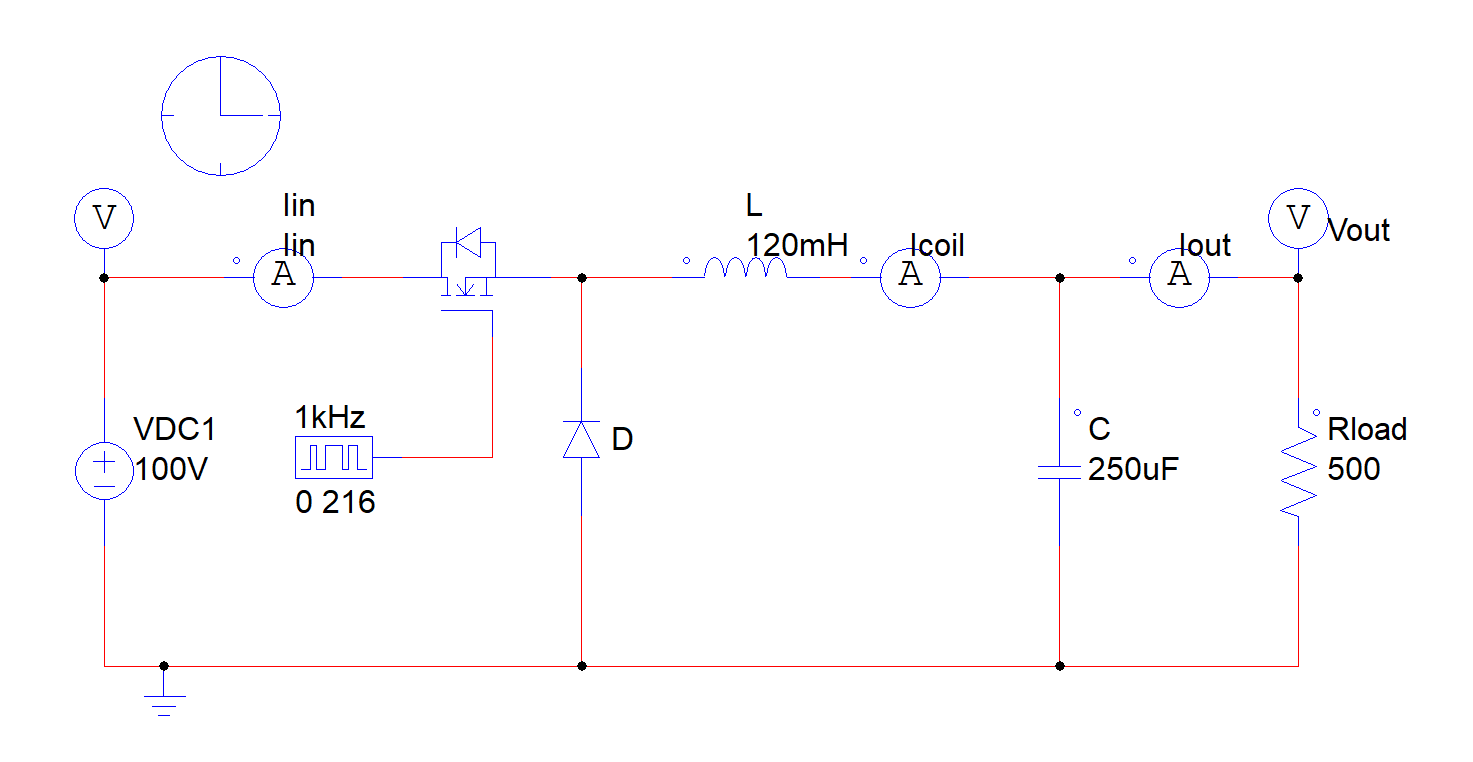
\includegraphics[width=0.8\linewidth,height=\textheight,keepaspectratio]{data/figures/buck_openLoop_schematic.png}

}

\caption{\label{fig-buck-schematic}Buck converter schematic in PSIM.}

\end{figure}%

\subsubsection{Simualtion results}\label{simualtion-results}

The once the stationari state is reached, the output voltage and
inductor current waveforms are shown in figures \#fig-buck-current and
\#fig-buck-voltage.

{\def\LTcaptype{none} % do not increment counter
\begin{longtable}[]{@{}lr@{}}
\toprule\noalign{}
Simulation parameter & Value \\
\midrule\noalign{}
\endhead
\bottomrule\noalign{}
\endlastfoot
Time step & 10e-6 \\
Total simulation time & 1.005 \\
Print time & 1 \\
Print step & 1 \\
\end{longtable}
}

\begin{figure}

\centering{

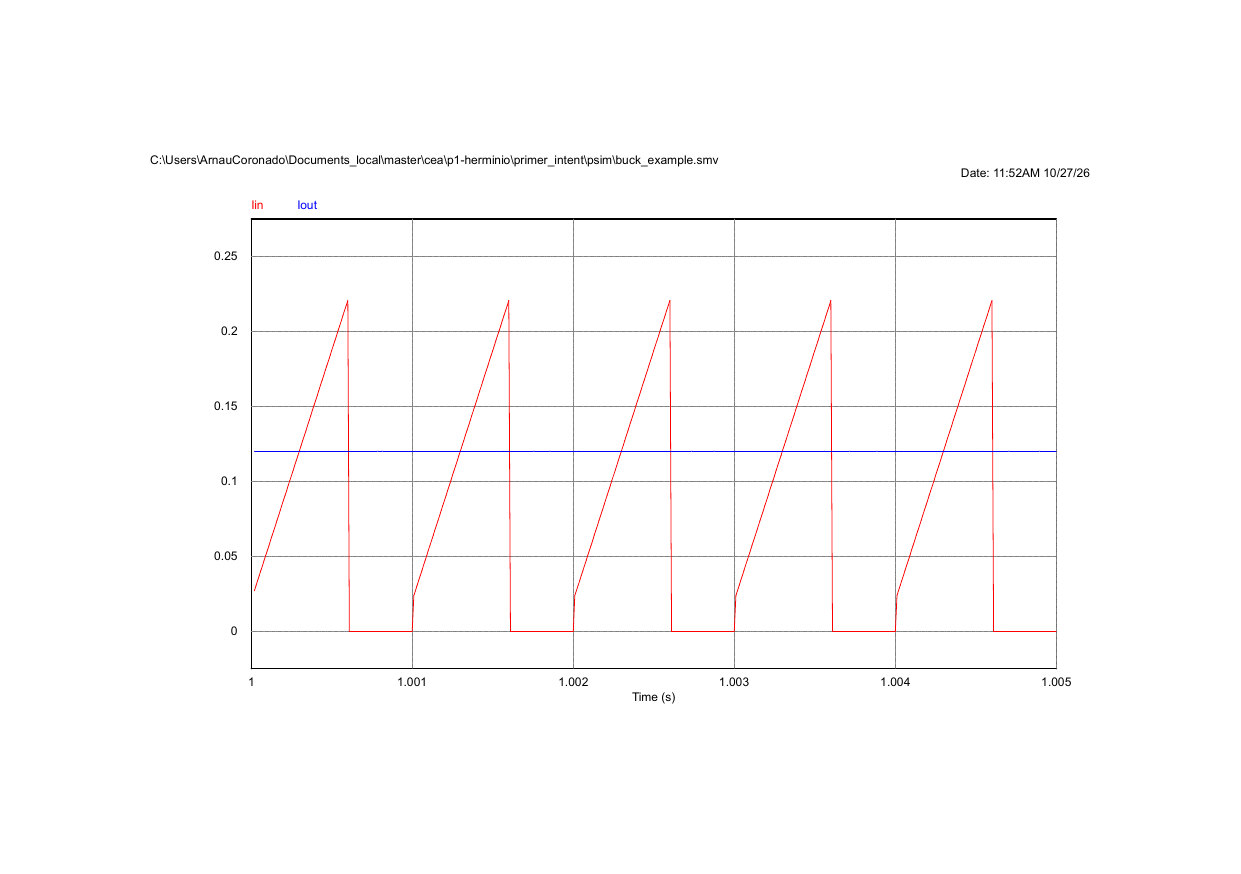
\includegraphics[width=0.9\linewidth,height=\textheight,keepaspectratio]{data/simview/buck_openLoop_Iin_Iout-1.png}

}

\caption{\label{fig-buck-current}Buck converter current waveforms.}

\end{figure}%

\begin{figure}

\centering{

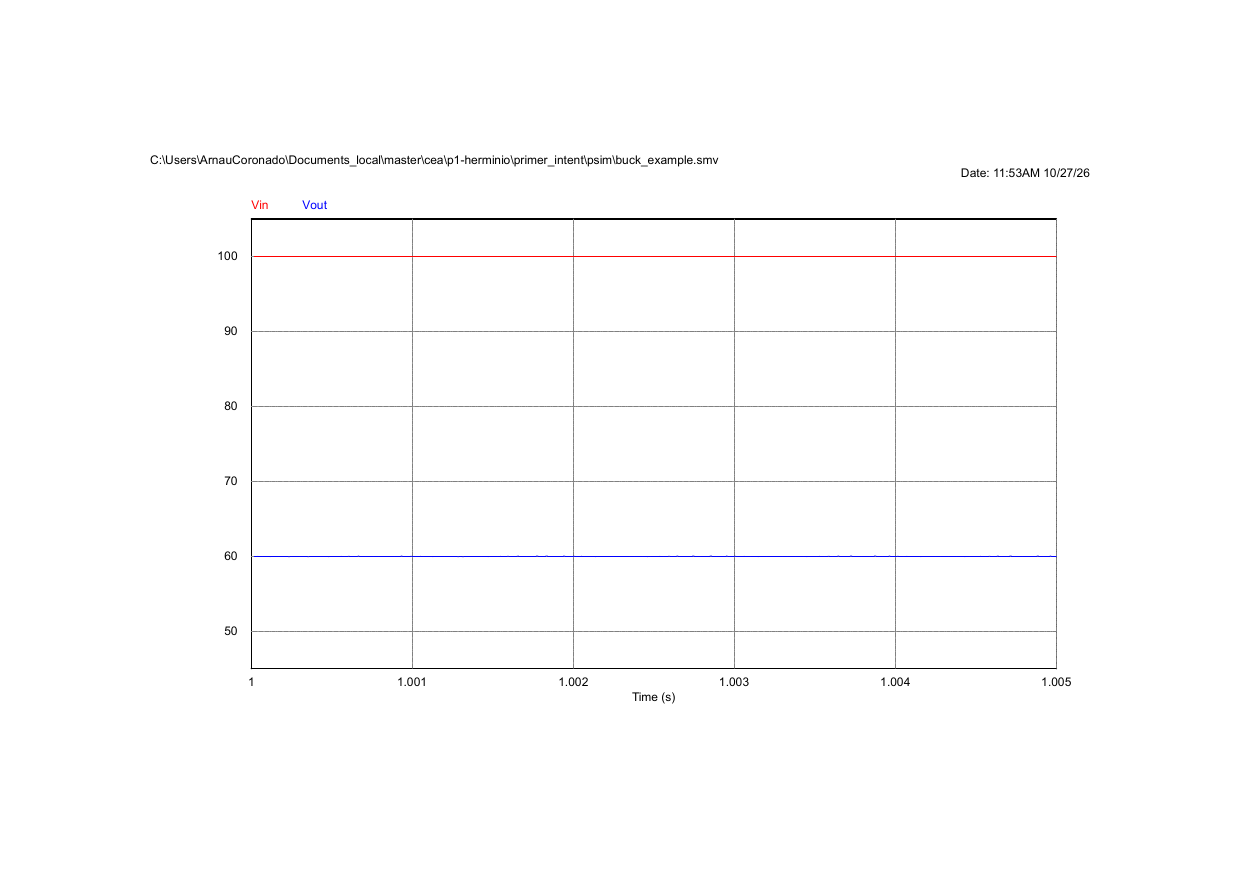
\includegraphics[width=0.9\linewidth,height=\textheight,keepaspectratio]{data/simview/buck_openLoop_Vin_Vout-1.png}

}

\caption{\label{fig-buck-voltage}Buck converter voltage waveforms.}

\end{figure}%

\subsubsection{Efficiency of the
circuit}\label{efficiency-of-the-circuit}

The input and output powers are calculated from the simulated voltage
and current measurements over the selected interval.

\begin{figure}

\centering{

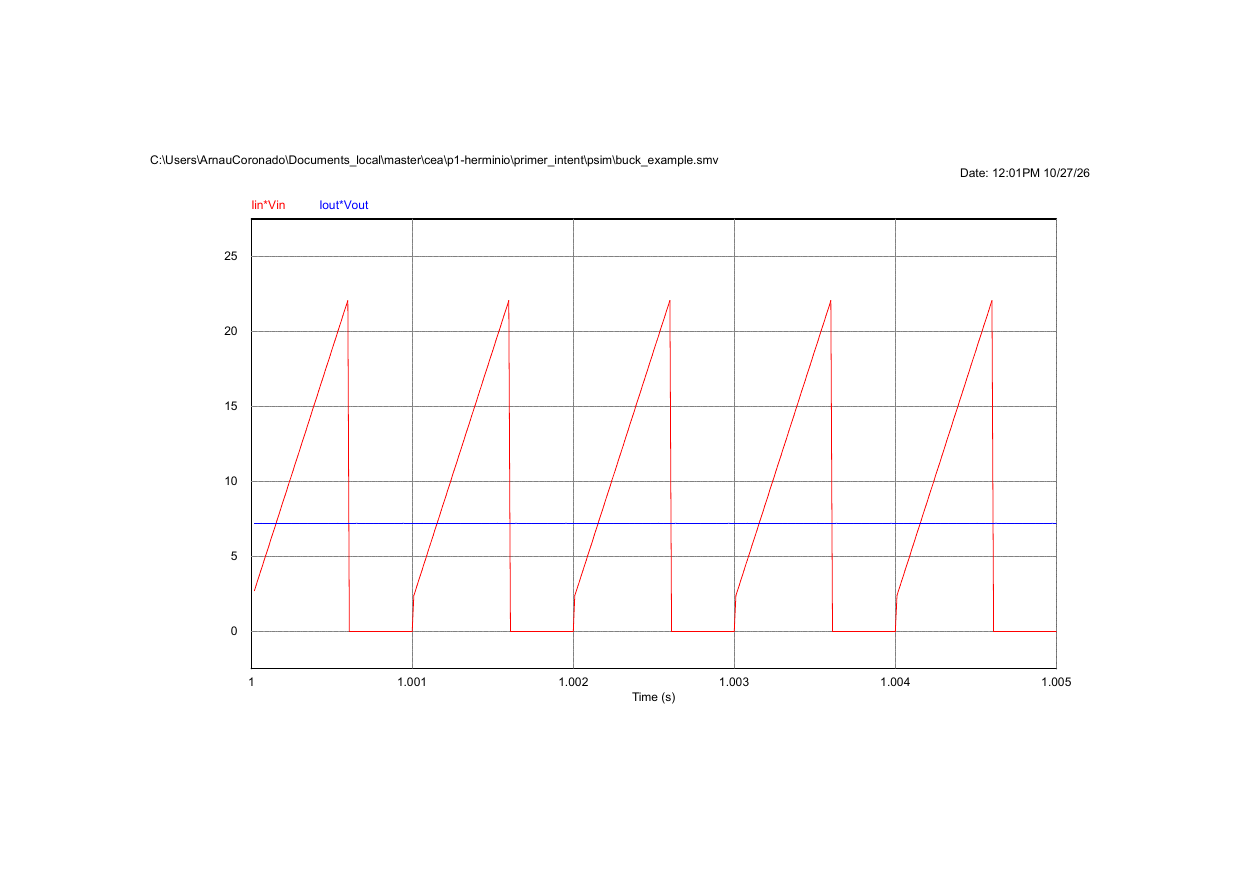
\includegraphics[width=0.9\linewidth,height=\textheight,keepaspectratio]{data/simview/buck_openLoop_IV-1.png}

}

\caption{\label{fig-buck-power}Buck converter instant power waveforms.}

\end{figure}%

\[
\begin{aligned}
\eta &= \frac{P_{out}}{P_{in}}\times100 \\
&= \frac{V_{out}I_{out}}{V_{in}I_{in}}\times100 \\
&= \frac{60 \times 0.12}{100 \times 0.072}\times100 \\
&= \frac{7.2}{7.2}\times100 \\
&= 100\%
\end{aligned}
\]

Because we are simulating an ideal converter, the efficiency is 100\%.

\subsection{Buck converter with
losses}\label{buck-converter-with-losses}

In the first place a PSIM schematic of the buck converter is designed in
the PSIM environment, but now the variables are left as parameters to be
able to change them in the simulation.

\begin{figure}

\centering{

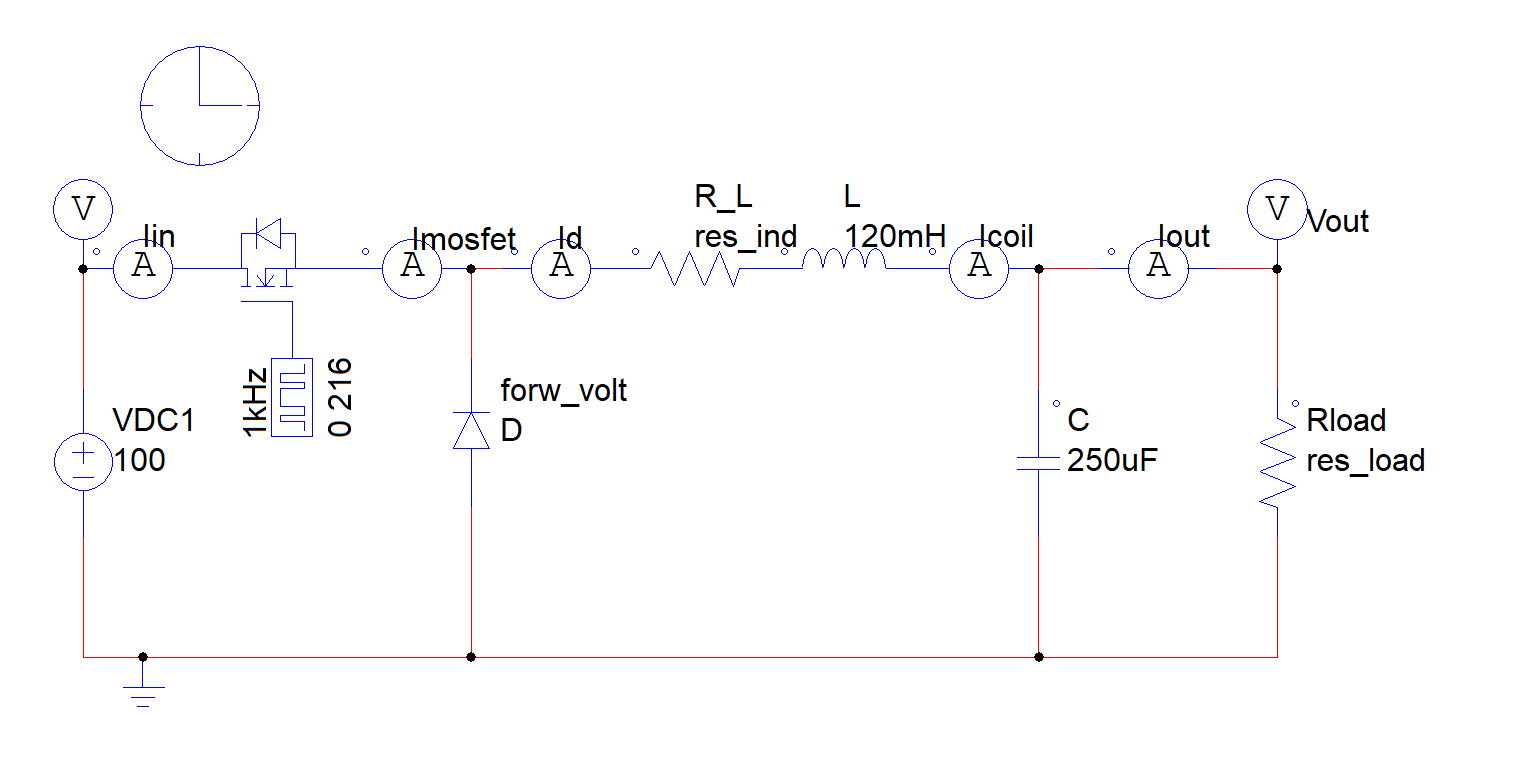
\includegraphics[width=0.9\linewidth,height=\textheight,keepaspectratio]{data/figures/buck_losses_schematic.png}

}

\caption{\label{fig-buck-losses-schematic}Buck converter with losses
schematic.}

\end{figure}%

This file can be exported to a Netlist File (Menu/Simulate/Generate
Netlist File).

\begin{Shaded}
\begin{Highlighting}[]
\NormalTok{.TIME 1E{-}005 1.005 1 1 0 0 0 0 0}
\NormalTok{.TI\_DMC\_VERSION 402 }
\NormalTok{VP Vin 1 }
\NormalTok{VP Vout 2 }
\NormalTok{VDC VDC1 1 0 100 0 0 }
\NormalTok{IP Icoil 3 4 }
\NormalTok{IP Iout 4 2 }
\NormalTok{C C 4 0 250uF 0 0 }
\NormalTok{L L 9 3 120mH 0 0 }
\NormalTok{DIODE D 0 8 forw\_volt 0 0 0 }
\NormalTok{MOSFET Q1 5 6 7 0 1 0 0 0 }
\NormalTok{R Rload 2 0 res\_load 0 }
\NormalTok{R R\_L 10 9 res\_ind 0 }
\NormalTok{IP Iin 1 5 }
\NormalTok{GATING G2 7 1kHz 2 0 216 }
\NormalTok{IP Imosfet 6 8 }
\NormalTok{IP Id 8 10 }
\end{Highlighting}
\end{Shaded}

The exported netlist can be simulated from the command line using PSIM's
\texttt{PsimCmd.exe} tool, without manually opening the schematic in the
graphical interface. This allows the simulation to be executed
programmatically, with the resulting output variables exported to a text
file for further analysis in Python.

\subsubsection{Inductor resistance}\label{inductor-resistance}

The following values are tested:

{\def\LTcaptype{none} % do not increment counter
\begin{longtable}[]{@{}ll@{}}
\toprule\noalign{}
Test & Load resistance \(R_L\) \\
\midrule\noalign{}
\endhead
\bottomrule\noalign{}
\endlastfoot
1 & \(0\ \Omega\) \\
2 & \(2\ \Omega\) \\
3 & \(10\ \Omega\) \\
\end{longtable}
}

The nominal load resistance is still \(R_{\text{load}} = 500\, \Omega\).

\subsubsection{Diode forward voltage}\label{diode-forward-voltage}

The following diode forward voltages are tested:

\[
V_F = 0\ V,\quad
1\ V,\quad
2\ V
\]

\subsubsection{Efficiency versus output
current}\label{efficiency-versus-output-current}

Three output-current conditions are considered:

\[
R_{load} = 500\ \Omega,\quad
250\ \Omega,\quad
125\ \Omega
\]

\subsubsection{Results}\label{results}

\begin{figure}[H]

{\centering 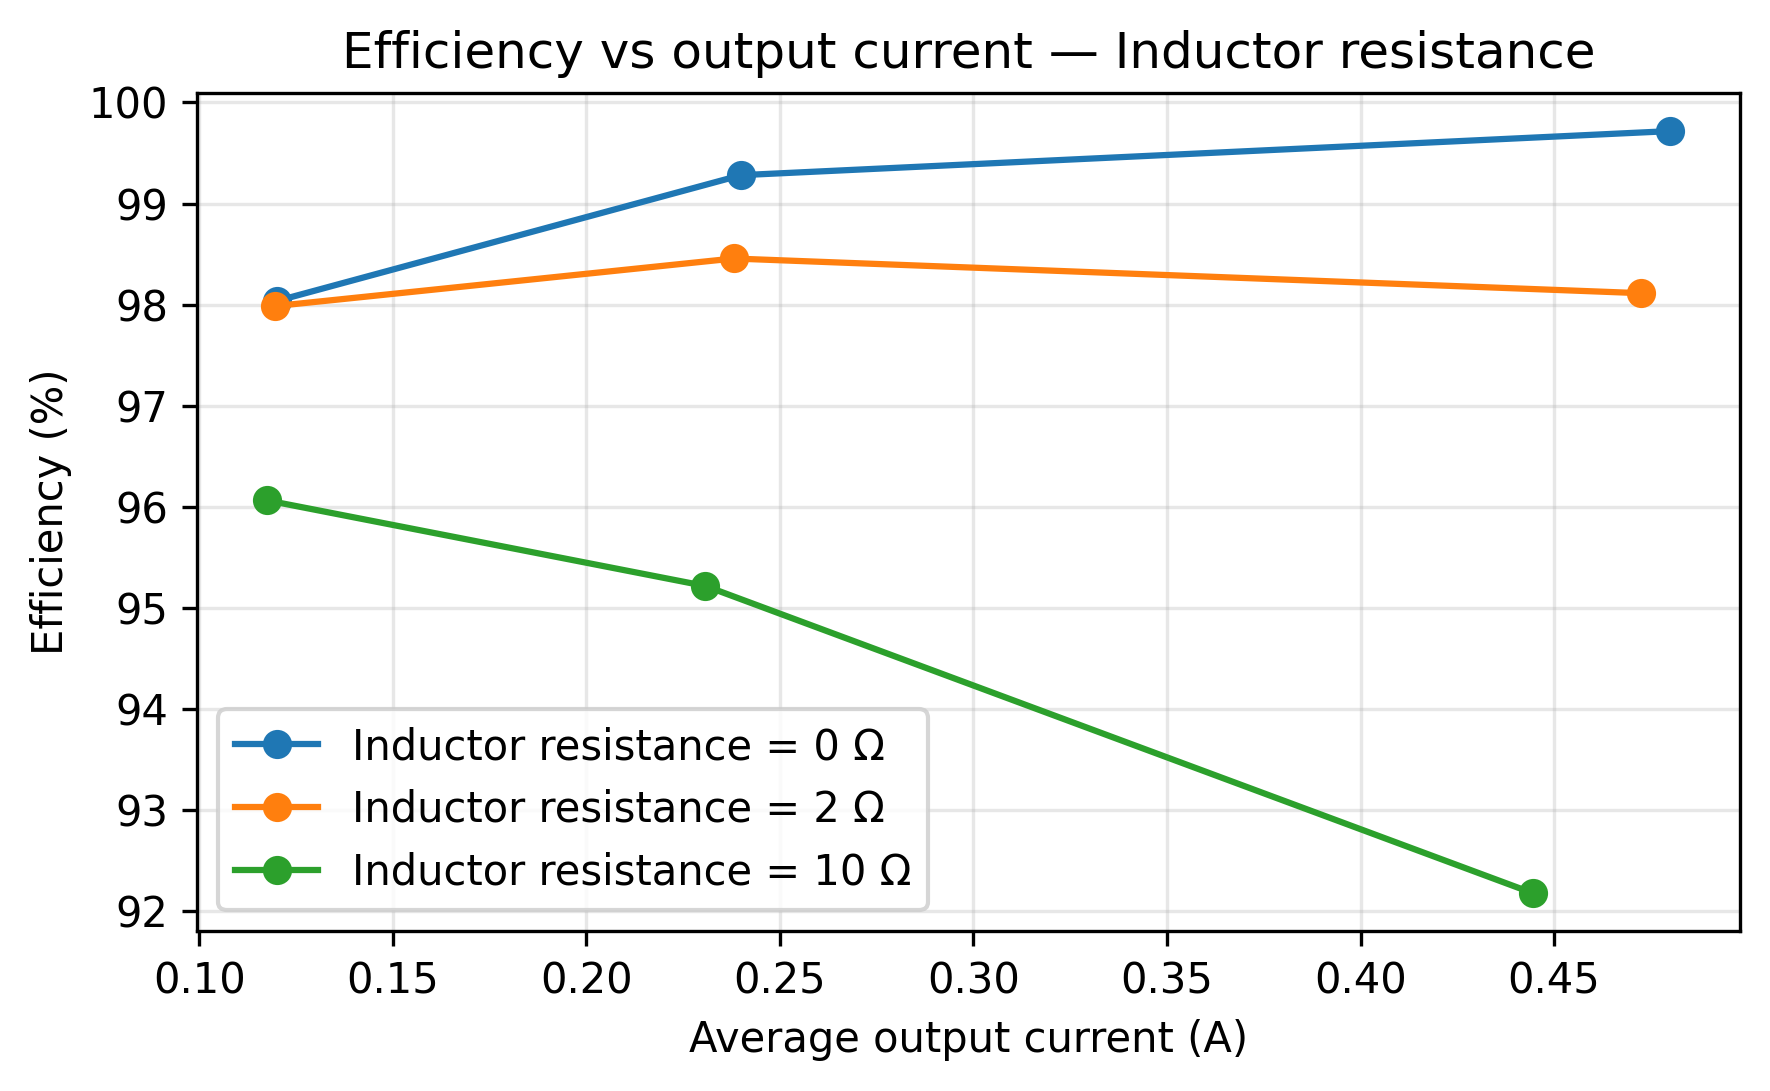
\includegraphics[width=0.75\linewidth,height=\textheight,keepaspectratio]{data/figures/buck_efficiency_inductor_resistance.png}

}

\caption{Efficiency versus output current for different inductor
resistances.}

\end{figure}%

\begin{figure}[H]

{\centering 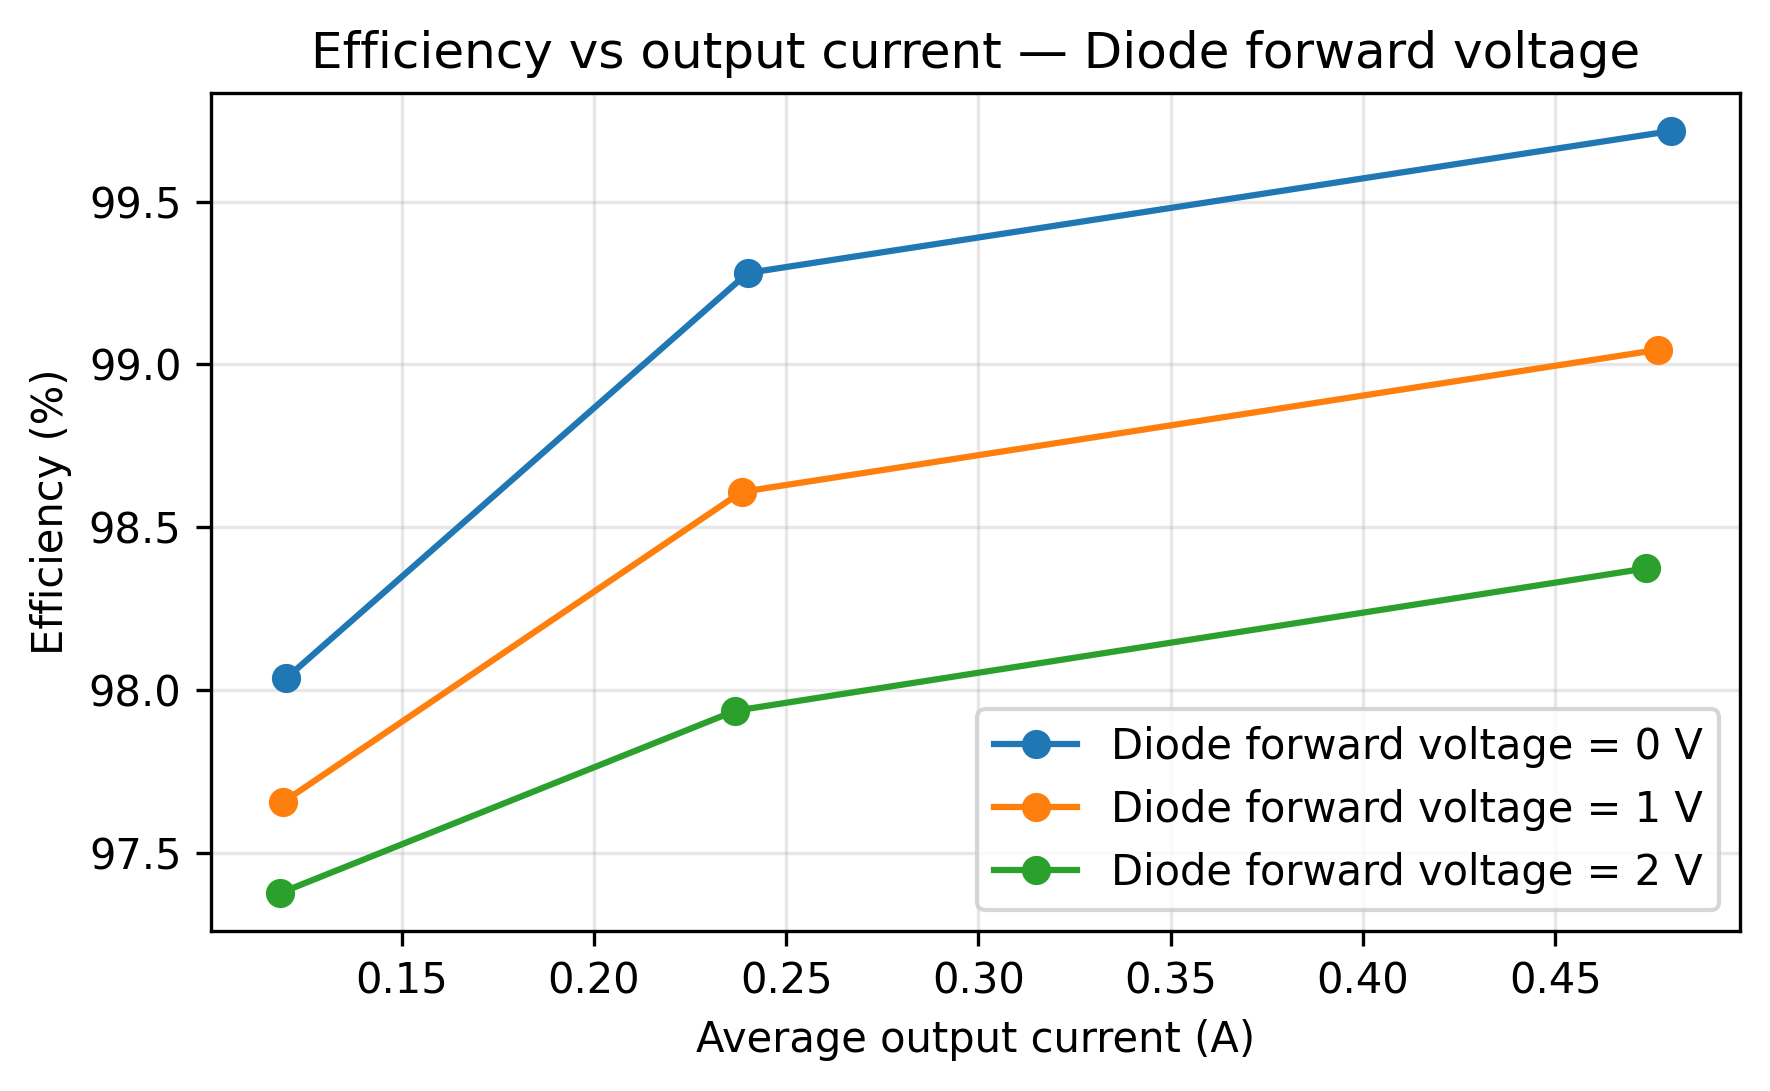
\includegraphics[width=0.75\linewidth,height=\textheight,keepaspectratio]{data/figures/buck_efficiency_diode_forward_voltage.png}

}

\caption{Efficiency versus output current for different diode forward
voltages.}

\end{figure}%

\subsubsection{Discussion}\label{discussion}

Increasing the inductor resistance increases conduction losses:

\[
P_L \approx I_L^2R_L
\]

Therefore, efficiency decreases as the inductor resistance increases,
particularly at higher output currents.

In the image it can be appreciated, however, that at ideal conditions
and low resistance, the increase in the output current increases the
efficiency. This is because the conduction losses are lower than the
switching losses, which are constant and independent of the output
current.

Increasing the diode forward voltage also increases conduction losses:

\[
P_D \approx V_F I_D
\]

Therefore, higher diode forward voltage produces lower efficiency.

Increasing the output current increases conduction losses in both the
inductor and the diode, which reduces efficiency.

\subsection{Buck converter with losses --- Closed
loop}\label{buck-converter-with-losses-closed-loop}

First the buck converter was designed in MODELICA.

\begin{figure}[H]

{\centering 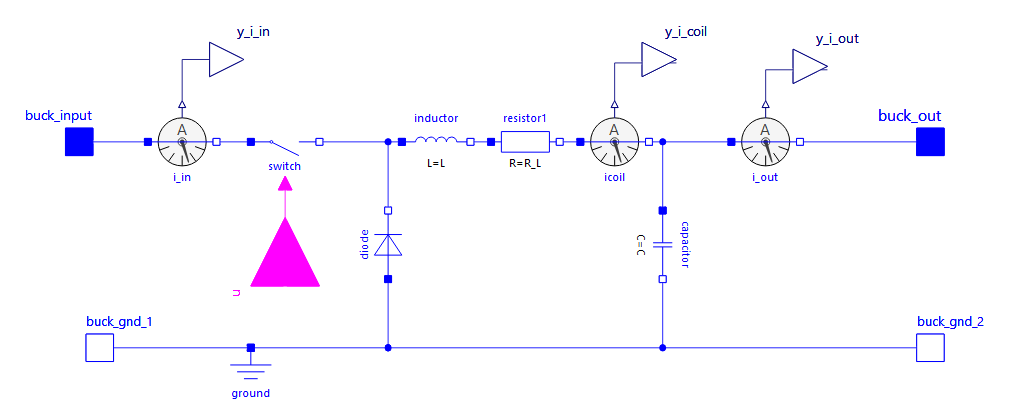
\includegraphics[width=0.75\linewidth,height=\textheight,keepaspectratio]{data/figures/buck_om.png}

}

\caption{Buck converter schematic.}

\end{figure}%

\subsubsection{P controller}\label{p-controller}

The output voltage is regulated to \(V_{\mathrm{ref}}=60\,\mathrm{V}\)
from a \(100\,\mathrm{V}\) input, giving \(D=0.6\). A proportional
controller \(G_c(s)=K_P\) is used, with \(K_P=0.01\).

\begin{figure}

\centering{

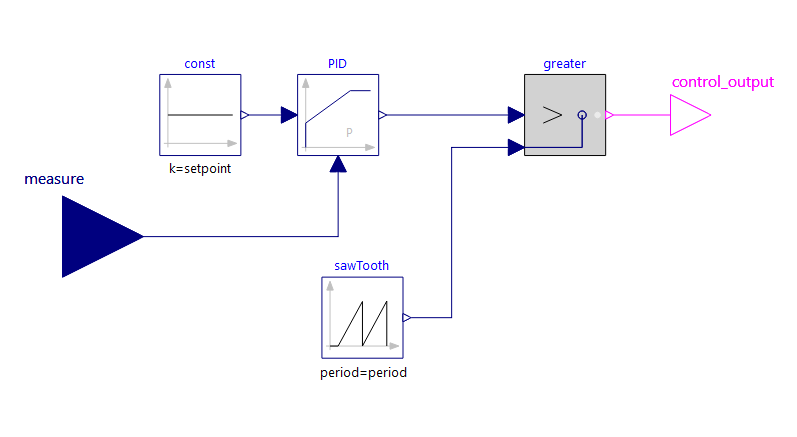
\includegraphics[width=0.75\linewidth,height=\textheight,keepaspectratio]{data/figures/controlP.png}

}

\caption{\label{fig-control-p}P controller.}

\end{figure}%

The buck converter and the P controller are connected in a closed-loop
configuration, as shown in the following figure.

\begin{figure}

\centering{

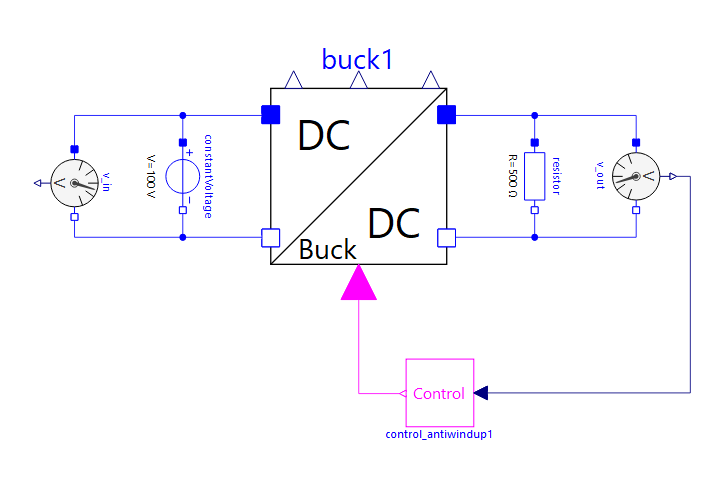
\includegraphics[width=0.75\linewidth,height=\textheight,keepaspectratio]{data/figures/buck_closedLoop_schematic.png}

}

\caption{\label{fig-buck-closed-loop-p}Closed-loop buck converter with P
controller.}

\end{figure}%

\begin{figure}

{\centering \pandocbounded{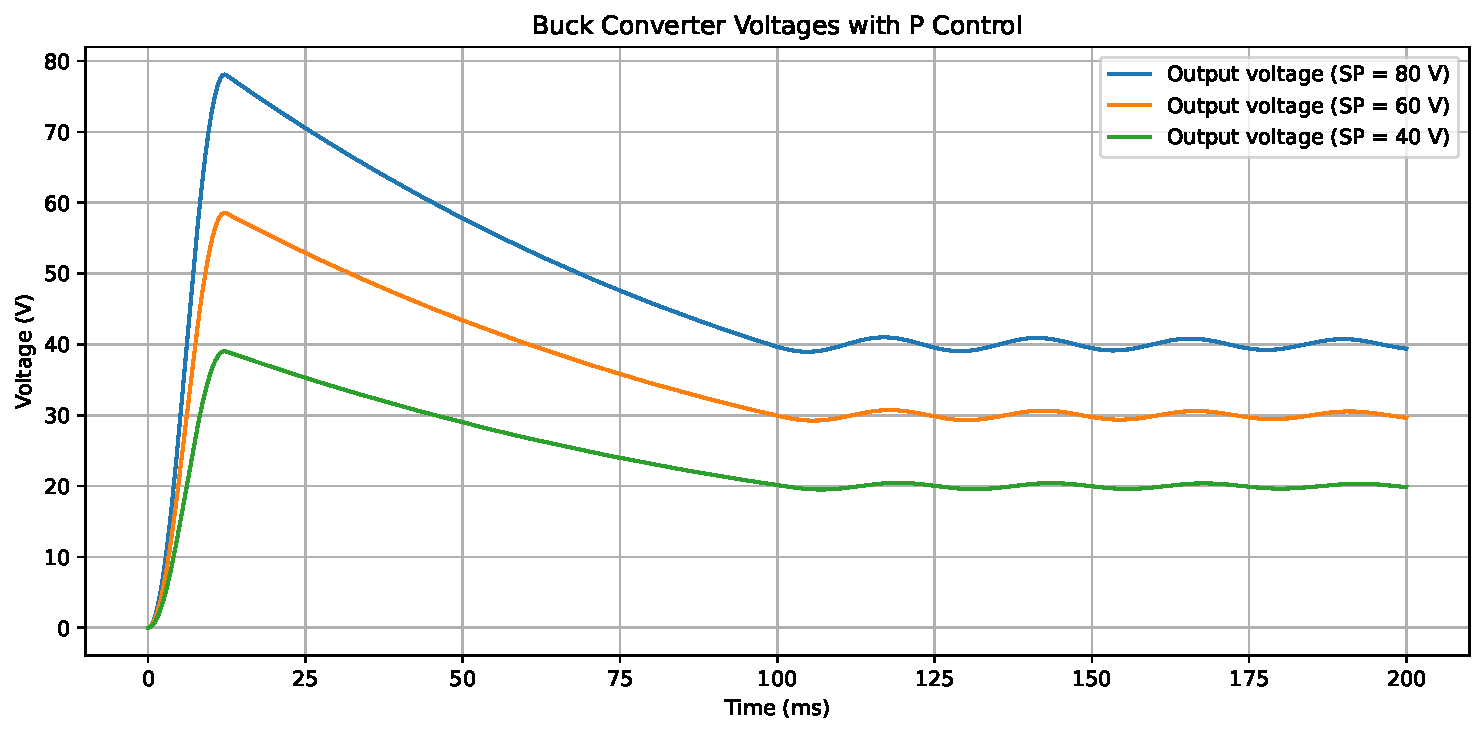
\includegraphics[keepaspectratio]{dcdc_report_files/figure-pdf/buck-closed-loop-p-output-1.pdf}}

}

\caption{Buck converter response using P control.}

\end{figure}%

{\def\LTcaptype{none} % do not increment counter
\begin{longtable}[]{@{}rrrr@{}}
\toprule\noalign{}
V\_ref & V\_out & Static error & Duty cycle \\
\midrule\noalign{}
\endhead
\bottomrule\noalign{}
\endlastfoot
80 V & 40 V & 40 V & 0.4 \\
60 V & 30 V & 30 V & 0.3 \\
40 V & 20 V & 20 V & 0.2 \\
\end{longtable}
}

A P controller generally produces a non-zero static error because a
finite error is required to generate the control action necessary to
maintain the output voltage.

\subsubsection{PI controller}\label{pi-controller}

The controller is changed to:

\[
G_c(s)=K_P+\frac{K_I}{s}
\]

Controller parameters:

{\def\LTcaptype{none} % do not increment counter
\begin{longtable}[]{@{}lr@{}}
\toprule\noalign{}
Parameter & Value \\
\midrule\noalign{}
\endhead
\bottomrule\noalign{}
\endlastfoot
K\_P & 0.01 \\
K\_I & 0.05 \\
\end{longtable}
}

The controller gains are adjusted to obtain a stable response with low
overshoot and negligible steady-state error.

Results:

{\def\LTcaptype{none} % do not increment counter
\begin{longtable}[]{@{}rrr@{}}
\toprule\noalign{}
V\_ref & V\_out & Static error \\
\midrule\noalign{}
\endhead
\bottomrule\noalign{}
\endlastfoot
40 V & 40 V & 0 V \\
60 V & 60 V & 0 V \\
80 V & 80 V & 0 V \\
\end{longtable}
}

\begin{figure}

{\centering \pandocbounded{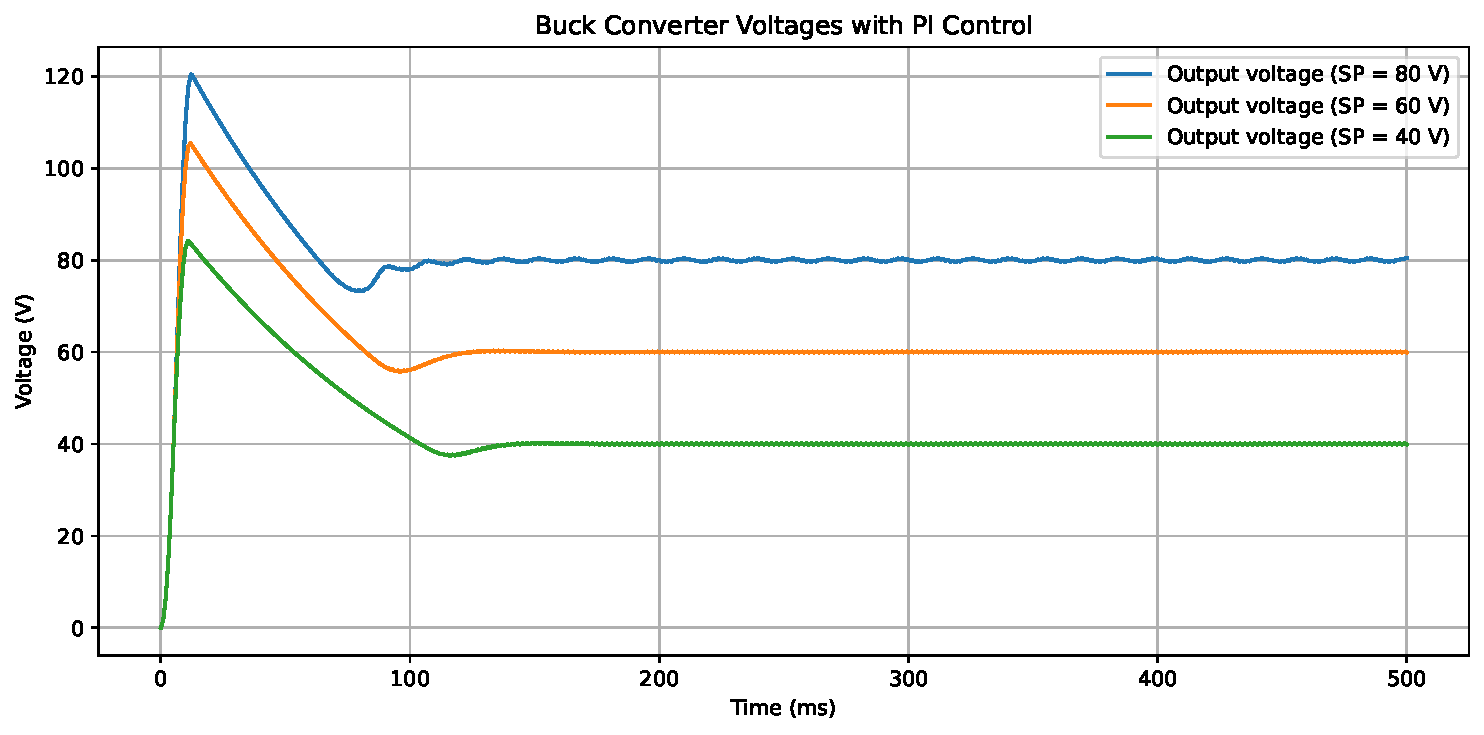
\includegraphics[keepaspectratio]{dcdc_report_files/figure-pdf/buck-closed-loop-pi-output-1.pdf}}

}

\caption{Buck converter response using PI control.}

\end{figure}%

\subsubsection{Setpoint change}\label{setpoint-change}

Apply a step change to the reference voltage.

{\def\LTcaptype{none} % do not increment counter
\begin{longtable}[]{@{}lr@{}}
\toprule\noalign{}
Parameter & Result \\
\midrule\noalign{}
\endhead
\bottomrule\noalign{}
\endlastfoot
Initial reference & \_\_\_\_\_\_ V \\
Final reference & \_\_\_\_\_\_ V \\
Rise time & \_\_\_\_\_\_ \\
Settling time & \_\_\_\_\_\_ \\
Overshoot & \_\_\_\_\_\_ \\
Final steady-state error & \_\_\_\_\_\_ \\
\end{longtable}
}

{[}INSERT SETPOINT RESPONSE HERE{]}

Figure 5.4 --- Response to a change in voltage reference.

\subsubsection{Line regulation}\label{line-regulation}

Change the input voltage while keeping the output reference constant.

{\def\LTcaptype{none} % do not increment counter
\begin{longtable}[]{@{}lr@{}}
\toprule\noalign{}
Parameter & Result \\
\midrule\noalign{}
\endhead
\bottomrule\noalign{}
\endlastfoot
Initial input voltage & \_\_\_\_\_\_ V \\
Final input voltage & \_\_\_\_\_\_ V \\
Output voltage before change & \_\_\_\_\_\_ V \\
Output voltage after settling & \_\_\_\_\_\_ V \\
\end{longtable}
}

{[}INSERT LINE REGULATION RESPONSE HERE{]}

Figure 5.5 --- Line regulation of the closed-loop buck converter.

\subsection{Boost converter --- Open
loop}\label{boost-converter-open-loop}

\subsubsection{Specifications}\label{specifications}

{\def\LTcaptype{none} % do not increment counter
\begin{longtable}[]{@{}lr@{}}
\toprule\noalign{}
Parameter & Value \\
\midrule\noalign{}
\endhead
\bottomrule\noalign{}
\endlastfoot
Input voltage & 100 V \\
Output voltage & 250 V \\
Maximum output current & 500 mA \\
Maximum output voltage ripple & 1 V \\
Maximum inductor current ripple & 500 mA \\
Switching frequency & 1 kHz \\
\end{longtable}
}

\subsubsection{Theoretical design}\label{theoretical-design-1}

Switching period:

\[
T_s=1\ ms
\]

For an ideal boost converter:

\[
D=1-\frac{V_{in}}{V_{out}}
=1-\frac{100}{250}
=0.6
\]

\[
T_{on}=0.6\ ms
\]

\[
T_{off}=0.4\ ms
\]

Load resistance:

\[
R_{load}=\frac{250}{0.5}=500\ \Omega
\]

Minimum inductance:

\[
L=
\frac{V_{in}D}
{\Delta I_Lf_s}
=
120\ mH
\]

Minimum capacitance:

\[
C\geq
\frac{I_{out}D}
{f_s\Delta V_{out}}
=
300\ \mu F
\]

Final design:

{\def\LTcaptype{none} % do not increment counter
\begin{longtable}[]{@{}lrr@{}}
\toprule\noalign{}
Parameter & Calculated & Selected \\
\midrule\noalign{}
\endhead
\bottomrule\noalign{}
\endlastfoot
Duty cycle & 0.60 & 0.60 \\
Switching period & 1 ms & 1 ms \\
Load resistance & 500 Ω & 500 Ω \\
Inductance & 120 mH & 120 mH \\
Capacitance & 300 µF & \_\_\_\_\_\_ \\
Switching frequency & 1 kHz & 1 kHz \\
\end{longtable}
}

\subsubsection{Simulation and results}\label{simulation-and-results}

{[}INSERT BOOST PSIM SCHEMATIC HERE{]}

Figure 6.1 --- Boost converter schematic.

{\def\LTcaptype{none} % do not increment counter
\begin{longtable}[]{@{}lrr@{}}
\toprule\noalign{}
Quantity & Theoretical & Simulated \\
\midrule\noalign{}
\endhead
\bottomrule\noalign{}
\endlastfoot
Average output voltage & 250 V & \_\_\_\_\_\_ \\
Maximum output voltage & --- & \_\_\_\_\_\_ \\
Minimum output voltage & --- & \_\_\_\_\_\_ \\
Output voltage ripple & ≤ 1 V & \_\_\_\_\_\_ \\
Maximum inductor current & --- & \_\_\_\_\_\_ \\
Minimum inductor current & --- & \_\_\_\_\_\_ \\
Inductor current ripple & ≤ 500 mA & \_\_\_\_\_\_ \\
\end{longtable}
}

{[}INSERT OUTPUT VOLTAGE AND INDUCTOR CURRENT WAVEFORMS HERE{]}

Figure 6.2 --- Boost converter steady-state waveforms.

\subsection{Buck-boost converter --- Open
loop}\label{buck-boost-converter-open-loop}

\subsubsection{Specifications}\label{specifications-1}

{\def\LTcaptype{none} % do not increment counter
\begin{longtable}[]{@{}lr@{}}
\toprule\noalign{}
Parameter & Value \\
\midrule\noalign{}
\endhead
\bottomrule\noalign{}
\endlastfoot
Input voltage & 100 V \\
Output voltage & -150 V \\
Maximum output current & 300 mA \\
Maximum output voltage ripple & 600 mV \\
Maximum inductor current ripple & 500 mA \\
Switching frequency & 1 kHz \\
\end{longtable}
}

\subsubsection{Theoretical design}\label{theoretical-design-2}

Switching period:

\[
T_s=1\ ms
\]

For an ideal inverting buck-boost converter:

\[
D=
\frac{|V_{out}|}
{V_{in}+|V_{out}|}
=
\frac{150}{100+150}
=
0.6
\]

Load resistance:

\[
R_{load}=
\frac{150}{0.3}
=
500\ \Omega
\]

Minimum inductance:

\[
L=
\frac{V_{in}D}
{\Delta I_Lf_s}
=
120\ mH
\]

Minimum capacitance:

\[
C\geq
\frac{I_{out}D}
{f_s\Delta V_{out}}
=
300\ \mu F
\]

Final design:

{\def\LTcaptype{none} % do not increment counter
\begin{longtable}[]{@{}lrr@{}}
\toprule\noalign{}
Parameter & Calculated & Selected \\
\midrule\noalign{}
\endhead
\bottomrule\noalign{}
\endlastfoot
Duty cycle & 0.60 & 0.60 \\
Switching period & 1 ms & 1 ms \\
Load resistance & 500 Ω & 500 Ω \\
Inductance & 120 mH & 120 mH \\
Capacitance & 300 µF & \_\_\_\_\_\_ \\
Switching frequency & 1 kHz & 1 kHz \\
\end{longtable}
}

\subsubsection{Simulation and results}\label{simulation-and-results-1}

{[}INSERT BUCK-BOOST PSIM SCHEMATIC HERE{]}

Figure 7.1 --- Buck-boost converter schematic.

{\def\LTcaptype{none} % do not increment counter
\begin{longtable}[]{@{}lrr@{}}
\toprule\noalign{}
Quantity & Theoretical & Simulated \\
\midrule\noalign{}
\endhead
\bottomrule\noalign{}
\endlastfoot
Average output voltage & -150 V & \_\_\_\_\_\_ \\
Maximum output voltage & --- & \_\_\_\_\_\_ \\
Minimum output voltage & --- & \_\_\_\_\_\_ \\
Output voltage ripple & ≤ 600 mV & \_\_\_\_\_\_ \\
Maximum inductor current & --- & \_\_\_\_\_\_ \\
Minimum inductor current & --- & \_\_\_\_\_\_ \\
Inductor current ripple & ≤ 500 mA & \_\_\_\_\_\_ \\
\end{longtable}
}

{[}INSERT OUTPUT VOLTAGE AND INDUCTOR CURRENT WAVEFORMS HERE{]}

Figure 7.2 --- Buck-boost converter steady-state waveforms.

\subsection{Flyback converter --- Open
loop}\label{flyback-converter-open-loop}

\subsubsection{Specifications}\label{specifications-2}

{\def\LTcaptype{none} % do not increment counter
\begin{longtable}[]{@{}lr@{}}
\toprule\noalign{}
Parameter & Value \\
\midrule\noalign{}
\endhead
\bottomrule\noalign{}
\endlastfoot
Input voltage & 12 V \\
Output voltage & 48 V \\
Maximum output current & 5 A \\
Maximum output voltage ripple & 10 mV \\
Transformer ratio N1/N2 & 100/200 \\
Magnetizing inductance & 100 µH \\
Switching frequency & 100 kHz \\
\end{longtable}
}

\subsubsection{Theoretical design}\label{theoretical-design-3}

Transformer ratio:

\[
\frac{N_1}{N_2}=0.5
\]

\[
\frac{N_2}{N_1}=2
\]

Switching period:

\[
T_s=10\ \mu s
\]

For an ideal flyback converter:

\[
V_{out}
=
\frac{N_2}{N_1}
\frac{D}{1-D}
V_{in}
\]

Therefore:

\[
D=
\frac{V_{out}}
{V_{out}+(N_2/N_1)V_{in}}
=
\frac{48}{48+2(12)}
=
0.667
\]

Load resistance:

\[
R_{load}=\frac{48}{5}=9.6\ \Omega
\]

Magnetizing inductance:

\[
L_m=100\ \mu H
\]

The output capacitance must be selected so that the simulated output
ripple remains below 10 mV.

\subsubsection{Simulation and results}\label{simulation-and-results-2}

{[}INSERT FLYBACK PSIM SCHEMATIC HERE{]}

Figure 8.1 --- Flyback converter schematic.

{\def\LTcaptype{none} % do not increment counter
\begin{longtable}[]{@{}lr@{}}
\toprule\noalign{}
Simulation parameter & Value \\
\midrule\noalign{}
\endhead
\bottomrule\noalign{}
\endlastfoot
Switching frequency & 100 kHz \\
Switching period & 10 µs \\
Time step & \_\_\_\_\_\_ \\
Total simulation time & \_\_\_\_\_\_ \\
Print time & \_\_\_\_\_\_ \\
Print step & 1 \\
\end{longtable}
}

Results:

{\def\LTcaptype{none} % do not increment counter
\begin{longtable}[]{@{}lrr@{}}
\toprule\noalign{}
Quantity & Specification & Simulated \\
\midrule\noalign{}
\endhead
\bottomrule\noalign{}
\endlastfoot
Average output voltage & 48 V & \_\_\_\_\_\_ \\
Output voltage ripple & ≤ 10 mV & \_\_\_\_\_\_ \\
Maximum primary current & --- & \_\_\_\_\_\_ \\
Output current & 5 A & \_\_\_\_\_\_ \\
\end{longtable}
}

{[}INSERT OUTPUT VOLTAGE WAVEFORM HERE{]}

Figure 8.2 --- Flyback converter output voltage.

{[}INSERT PRIMARY/MAGNETIZING CURRENT WAVEFORM HERE{]}

Figure 8.3 --- Flyback converter magnetizing current.

{[}INSERT SWITCH WAVEFORM HERE{]}

Figure 8.4 --- Flyback converter switch waveform.

\subsection{Forward converter --- Open
loop}\label{forward-converter-open-loop}

\subsubsection{Specifications}\label{specifications-3}

{\def\LTcaptype{none} % do not increment counter
\begin{longtable}[]{@{}lr@{}}
\toprule\noalign{}
Parameter & Value \\
\midrule\noalign{}
\endhead
\bottomrule\noalign{}
\endlastfoot
Input voltage & 10 V \\
Output voltage & 48 V \\
Maximum output current & 10 A \\
Maximum output voltage ripple & 50 mV \\
Transformer ratio N1/N2 & 10/100 \\
Output inductance & 400 µH \\
Maximum inductor current ripple & 2 A \\
Switching frequency & 40 kHz \\
\end{longtable}
}

\subsubsection{Theoretical design}\label{theoretical-design-4}

Transformer ratio:

\[
\frac{N_1}{N_2}=0.1
\]

\[
\frac{N_2}{N_1}=10
\]

Switching period:

\[
T_s=25\ \mu s
\]

For an ideal forward converter:

\[
V_{out}
=
D
\frac{N_2}{N_1}
V_{in}
\]

Therefore:

\[
D=
\frac{48}{10(10)}
=
0.48
\]

Load resistance:

\[
R_{load}
=
\frac{48}{10}
=
4.8\ \Omega
\]

Given:

\[
L=400\ \mu H
\]

The secondary voltage during the ON interval is:

\[
V_{sec}
=
\frac{N_2}{N_1}V_{in}
=
100\ V
\]

The inductor voltage is:

\[
V_L=V_{sec}-V_{out}=52\ V
\]

Therefore:

\[
\Delta I_L=
\frac{V_LD}{Lf_s}
=
1.56\ A
\]

Since:

\[
1.56\ A < 2\ A
\]

the current-ripple specification is satisfied theoretically.

Minimum output capacitance:

\[
C\geq
\frac{\Delta I_L}
{8f_s\Delta V_{out}}
\approx97.5\ \mu F
\]

Final design:

{\def\LTcaptype{none} % do not increment counter
\begin{longtable}[]{@{}lrr@{}}
\toprule\noalign{}
Parameter & Calculated & Selected \\
\midrule\noalign{}
\endhead
\bottomrule\noalign{}
\endlastfoot
Duty cycle & 0.48 & 0.48 \\
Switching period & 25 µs & 25 µs \\
Load resistance & 4.8 Ω & 4.8 Ω \\
Inductance & 400 µH & 400 µH \\
Capacitance & ≥ 97.5 µF & \_\_\_\_\_\_ \\
Switching frequency & 40 kHz & 40 kHz \\
\end{longtable}
}

\subsubsection{Simulation and results}\label{simulation-and-results-3}

{[}INSERT FORWARD PSIM SCHEMATIC HERE{]}

Figure 9.1 --- Forward converter schematic.

{\def\LTcaptype{none} % do not increment counter
\begin{longtable}[]{@{}lr@{}}
\toprule\noalign{}
Simulation parameter & Value \\
\midrule\noalign{}
\endhead
\bottomrule\noalign{}
\endlastfoot
Switching frequency & 40 kHz \\
Switching period & 25 µs \\
Time step & \_\_\_\_\_\_ \\
Total simulation time & \_\_\_\_\_\_ \\
Print time & \_\_\_\_\_\_ \\
Print step & 1 \\
\end{longtable}
}

Results:

{\def\LTcaptype{none} % do not increment counter
\begin{longtable}[]{@{}lrr@{}}
\toprule\noalign{}
Quantity & Specification & Simulated \\
\midrule\noalign{}
\endhead
\bottomrule\noalign{}
\endlastfoot
Average output voltage & 48 V & \_\_\_\_\_\_ \\
Maximum output voltage & --- & \_\_\_\_\_\_ \\
Minimum output voltage & --- & \_\_\_\_\_\_ \\
Output voltage ripple & ≤ 50 mV & \_\_\_\_\_\_ \\
Maximum inductor current & --- & \_\_\_\_\_\_ \\
Minimum inductor current & --- & \_\_\_\_\_\_ \\
Inductor current ripple & ≤ 2 A & \_\_\_\_\_\_ \\
\end{longtable}
}

{[}INSERT OUTPUT VOLTAGE WAVEFORM HERE{]}

Figure 9.2 --- Forward converter output voltage.

{[}INSERT INDUCTOR CURRENT WAVEFORM HERE{]}

Figure 9.3 --- Forward converter inductor current.

{[}INSERT SWITCH AND TRANSFORMER WAVEFORMS HERE{]}

Figure 9.4 --- Forward converter switching and transformer waveforms.

\section{Overall results}\label{overall-results}

{\def\LTcaptype{none} % do not increment counter
\begin{longtable}[]{@{}
  >{\raggedright\arraybackslash}p{(\linewidth - 16\tabcolsep) * \real{0.0882}}
  >{\raggedleft\arraybackslash}p{(\linewidth - 16\tabcolsep) * \real{0.1176}}
  >{\raggedleft\arraybackslash}p{(\linewidth - 16\tabcolsep) * \real{0.1176}}
  >{\raggedleft\arraybackslash}p{(\linewidth - 16\tabcolsep) * \real{0.1176}}
  >{\raggedleft\arraybackslash}p{(\linewidth - 16\tabcolsep) * \real{0.1176}}
  >{\raggedleft\arraybackslash}p{(\linewidth - 16\tabcolsep) * \real{0.1176}}
  >{\raggedleft\arraybackslash}p{(\linewidth - 16\tabcolsep) * \real{0.1176}}
  >{\raggedleft\arraybackslash}p{(\linewidth - 16\tabcolsep) * \real{0.1176}}
  >{\raggedright\arraybackslash}p{(\linewidth - 16\tabcolsep) * \real{0.0882}}@{}}
\toprule\noalign{}
\begin{minipage}[b]{\linewidth}\raggedright
Converter
\end{minipage} & \begin{minipage}[b]{\linewidth}\raggedleft
V\_in
\end{minipage} & \begin{minipage}[b]{\linewidth}\raggedleft
V\_out
\end{minipage} & \begin{minipage}[b]{\linewidth}\raggedleft
D
\end{minipage} & \begin{minipage}[b]{\linewidth}\raggedleft
L
\end{minipage} & \begin{minipage}[b]{\linewidth}\raggedleft
C
\end{minipage} & \begin{minipage}[b]{\linewidth}\raggedleft
f\_s
\end{minipage} & \begin{minipage}[b]{\linewidth}\raggedleft
Ripple
\end{minipage} & \begin{minipage}[b]{\linewidth}\raggedright
Result
\end{minipage} \\
\midrule\noalign{}
\endhead
\bottomrule\noalign{}
\endlastfoot
Buck & 100 V & 60 V & 0.60 & 120 mH & 250 µF & 1 kHz & \_\_\_\_\_\_ &
\_\_\_\_\_\_ \\
Boost & 100 V & 250 V & 0.60 & 120 mH & \_\_\_\_\_\_ & 1 kHz &
\_\_\_\_\_\_ & \_\_\_\_\_\_ \\
Buck-boost & 100 V & -150 V & 0.60 & 120 mH & \_\_\_\_\_\_ & 1 kHz &
\_\_\_\_\_\_ & \_\_\_\_\_\_ \\
Flyback & 12 V & 48 V & 0.667 & 100 µH & \_\_\_\_\_\_ & 100 kHz &
\_\_\_\_\_\_ & \_\_\_\_\_\_ \\
Forward & 10 V & 48 V & 0.48 & 400 µH & \_\_\_\_\_\_ & 40 kHz &
\_\_\_\_\_\_ & \_\_\_\_\_\_ \\
\end{longtable}
}

\section{Conclusions}\label{conclusions}

\subsection{Buck converter}\label{buck-converter}

{[}WRITE CONCLUSION HERE{]}

\subsection{Non-ideal components}\label{non-ideal-components}

{[}WRITE CONCLUSION HERE{]}

\subsection{Open-loop versus closed-loop
operation}\label{open-loop-versus-closed-loop-operation}

{[}WRITE CONCLUSION HERE{]}

\subsection{P versus PI control}\label{p-versus-pi-control}

{[}WRITE CONCLUSION HERE{]}

\subsection{Boost converter}\label{boost-converter}

{[}WRITE CONCLUSION HERE{]}

\subsection{Buck-boost converter}\label{buck-boost-converter}

{[}WRITE CONCLUSION HERE{]}

\subsection{Flyback converter}\label{flyback-converter}

{[}WRITE CONCLUSION HERE{]}

\subsection{Forward converter}\label{forward-converter}

{[}WRITE CONCLUSION HERE{]}

\subsection{Overall conclusion}\label{overall-conclusion}

{[}WRITE FINAL CONCLUSION HERE{]}

\section{APPENDIX A --- POWER AND EFFICIENCY
CALCULATIONS}\label{appendix-a-power-and-efficiency-calculations}

Input power:

\[
P_{in}=AVG(V_{in}I_{in})
\]

Output power:

\[
P_{out}=AVG(V_{out}I_{out})
\]

Efficiency:

\[
\eta=
\frac{P_{out}}{P_{in}}\times100
\]

The measurements must be performed during steady-state operation.

The averaging interval should contain an integer number of switching
periods.

For the 1 kHz converters:

\[
T_s=1\ ms
\]

For example, a 10 ms averaging interval contains ten switching periods.

For the flyback converter:

\[
T_s=10\ \mu s
\]

For the forward converter:

\[
T_s=25\ \mu s
\]

\end{document}
